\documentclass{beamer}
\usepackage[utf8]{inputenc}
\usepackage{graphicx}
\usepackage{amsmath}
\usepackage{amssymb} % Para símbolos matemáticos
\usepackage{booktabs} % Para tabelas mais bonitas

\title{Análise e Controle Avançado de um Reator Químico}
\author{Lucas William Junges}
\institute{Universidade Federal de Santa Catarina (UFSC)}
\date{\today}

\usetheme{AnnArbor}
\usecolortheme{default}

\begin{document}

\begin{frame}
    \titlepage
\end{frame}

\begin{frame}{O Processo: Reator Químico}
    \begin{columns}[T]
        \begin{column}{0.5\textwidth}
            \textbf{Objetivo:} Controlar a concentração de Cyclopentenol (\(C_b\)) em um reator de agitação contínua.
            \vspace{1em}
            
            \textbf{Reações:}
            \[ A \xrightarrow{k_1} B \xrightarrow{k_2} C \]
            \[ 2A \xrightarrow{k_3} D\]
            
            \textbf{Dinâmica (Não Linear):}
            {\tiny
            \begin{align*}
            \frac{dC_a}{dt} &= -k_1 C_a - k_3 C_a^2 + u(C_{af} - C_a) \\
            \frac{dC_b}{dt} &= k_1 C_a - k_2 C_b - u C_b
            \end{align*}
            }
            \vspace{1em}
            \textbf{Variáveis:}
            \begin{itemize}
                \item Manipulada: \(u = F/V\)
                \item Perturbação: \(C_{af}\)
            \end{itemize}
        \end{column}
        \begin{column}{0.5\textwidth}
            \begin{figure}
                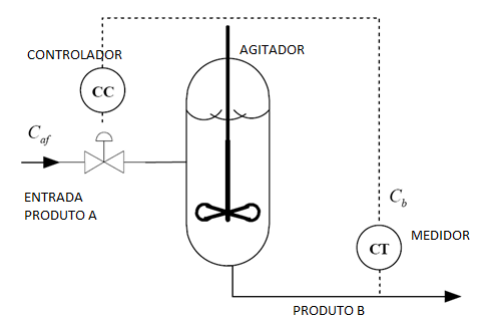
\includegraphics[width=\textwidth]{Imagens/Reator.png}
                \caption{Diagrama do Reator Químico.}
            \end{figure}
        \end{column}
    \end{columns}
\end{frame}

% --- PARTE 1 ---
\section{Parte 1: Análise e Controle PI por Alocação de Polos}

\begin{frame}{Parte 1: Análise e Alocação de Polos}
    \begin{block}{Roteiro}
        \begin{enumerate}
            \item Análise do sistema em equilíbrio para entender o comportamento estático.
            \item Linearização do modelo em um ponto de operação para permitir o projeto clássico.
            \item Projeto de um controlador PI via Alocação de Polos para atender especificações de desempenho.
            \item Validação do controle no sistema não linear e análise do efeito da discretização.
        \end{enumerate}
    \end{block}
\end{frame}

\begin{frame}{Linearização e Projeto do Controlador PI}
    \begin{columns}[T]
        \begin{column}{0.6\textwidth}
            \textbf{Ponto de Operação:}
            \begin{itemize}
                \item \( \overline{u} = 1 \) min\(^{-1}\)
                \item \( \overline{C}_{af} = 5.1 \) mol/L
                \item Resulta em: \( \overline{C}_a = 0.719 \), \( \overline{C}_b = 2.345 \)
            \end{itemize}
            
            \textbf{Modelo Linearizado:}
            {\tiny
            \begin{align*}
            \Delta\dot{C}_a &= -7.17 \Delta C_a + \Delta C_{af} + 4.38 \Delta u \\
            \Delta\dot{C}_b &= 6.01 \Delta C_a -1.84 \Delta C_b - 2.35 \Delta u
            \end{align*}
            }
            
            \textbf{Controlador PI (Alocação de Polos):}
            \begin{itemize}
                \item \textbf{Objetivo:} \(t_{5\%} \approx 1.6\) min, Pico \(< 5\%\).
                \item \textbf{Controlador:} \( C(s) = 1.85 \frac{s + 1.92}{s} \)
                \item \textbf{Filtro:} \( F_r(s) = \frac{1.92}{s + 1.92} \) para cancelar o zero e evitar overshoot.
            \end{itemize}
        \end{column}
        \begin{column}{0.4\textwidth}
            \begin{figure}
                \includegraphics[width=\textwidth]{{"Trabalho 1 Sistemas de Controle/figura15"}.png}
                \caption{Resposta ao degrau com filtro.}
            \end{figure}
            \begin{figure}
                \includegraphics[width=\textwidth]{{"Trabalho 1 Sistemas de Controle/figura16"}.png}
                \caption{Rejeição à perturbação.}
            \end{figure}
        \end{column}
    \end{columns}
\end{frame}

% --- PARTE 2 ---
\section{Parte 2: Controle Avançado por Lugar das Raízes}

\begin{frame}{Parte 2: Controle Avançado por LR}
    \begin{block}{Roteiro}
        \begin{enumerate}
            \item Projeto de um controlador mais complexo (PID) via Lugar das Raízes (LR) para o modelo de 2ª ordem.
            \item Comparação de desempenho: PI vs. PID-LR.
            \item Melhoria do sistema com controle Feedforward para rejeição de perturbações.
            \item Análise de robustez e simulação em cenário com ruído.
        \end{enumerate}
    \end{block}
\end{frame}

\begin{frame}{Projeto via Lugar das Raízes e Comparação}
    \begin{columns}[T]
        \begin{column}{0.55\textwidth}
            \textbf{Função de Transferência (\(C_b/u\)):}
            \[ G_{yu}(s) = \frac{-2.35(s-4.01)}{(s + 1.84)(s + 7.17)} \]
            \textit{Nota: A presença de um zero no semiplano direito (ZSD) impõe limitações de desempenho.}
            
            \textbf{Controlador (PID via LR):}
            \[ C(s) = \frac{5.29(s+3.83)^2}{s(s+20)} \]
            \textit{Projetado para os mesmos polos dominantes da Parte 1.}
            
            \textbf{Filtro de Referência:}
            \[ F_r(s) = \left(\frac{3.83}{s+3.83}\right)^2 \]
        \end{column}
        \begin{column}{0.45\textwidth}
            \begin{figure}
                \includegraphics[width=\textwidth]{{"Trabalho 2 Sistemas de Controle/Imagens/1B/1BComparacaoPILR"}.png}
                \caption{Comparativo: PI (azul) vs. PID por LR (vermelho).}
            \end{figure}
        \end{column}
    \end{columns}
    \vspace{1em}
    \textbf{Discussão:} O controlador PID projetado por LR mostra uma resposta mais suave e menos oscilatória que o PI, sendo mais adequado para a dinâmica de segunda ordem do sistema.
\end{frame}

\begin{frame}{Melhorando a Rejeição a Perturbações com Feedforward}
    \textbf{Estratégia:} Medir a perturbação (\(C_{af}\)) e agir proativamente para cancelar seu efeito.
    
    \textbf{Controlador Feedforward (\(C_{ff}\)):}
    \[ C_{ff}(s) = \frac{G_{pert}(s)}{G_{proc}(s)} = \frac{G_{C_b/C_{af}}(s)}{G_{C_b/u}(s)} \]
    Isso resulta em um controlador instável. A solução prática é usar uma aproximação estática:
    \[ C_{ff} \approx -0.4 \]
    
    \begin{columns}[T]
        \begin{column}{0.5\textwidth}
            \begin{figure}
                \includegraphics[width=\textwidth]{{"Trabalho 2 Sistemas de Controle/image3"}.png}
                \caption{Resposta à perturbação \textbf{sem} Feedforward.}
            \end{figure}
        \end{column}
        \begin{column}{0.5\textwidth}
            \begin{figure}
                \includegraphics[width=\textwidth]{{"Trabalho 2 Sistemas de Controle/image2"}.png}
                \caption{Resposta à perturbação \textbf{com} Feedforward.}
            \end{figure}
        \end{column}
    \end{columns}
    
    \textbf{Resultado:} A rejeição à perturbação é drasticamente melhorada, com o desvio na saída sendo quase eliminado.
\end{frame}

% --- PARTE 3 ---
\section{Parte 3: Lidando com Atraso de Medição}

\begin{frame}{Parte 3: O Desafio do Atraso de Tempo}
    \begin{block}{O Problema}
        \begin{itemize}
            \item Na prática, a medição de \(C_b\) não é instantânea. Existe um \textbf{atraso de transporte de 3 minutos}.
            \item A função de transferência do processo se torna: \( G_p(s)e^{-3s} \).
            \item O atraso adiciona uma fase negativa, que severamente degrada a estabilidade e o desempenho de controladores convencionais.
        \end{itemize}
    \end{block}
    
    \begin{block}{A Solução: Preditor de Smith}
        Uma estrutura de controle que utiliza um modelo do processo para "prever" a saída, efetivamente removendo o atraso da malha de realimentação e permitindo um controle mais agressivo e estável.
    \end{block}
\end{frame}

% --- CONCLUSÕES ---
\section{Conclusões e Perguntas}

\begin{frame}{Conclusões e Trabalhos Futuros}
    \begin{block}{Conclusões}
        \begin{itemize}
            \item A complexidade do controlador deve ser adequada à do processo (PI para 1ª ordem, PID para 2ª ordem).
            \item O controle Feedforward é uma ferramenta poderosa para rejeição de perturbações mensuráveis.
            \item Atrasos de tempo são um desafio significativo que requerem estratégias de controle específicas como o Preditor de Smith.
            \item A linearização é uma ferramenta essencial, mas suas limitações devem ser respeitadas, especialmente longe do ponto de operação.
        \end{itemize}
    \end{block}
    
    \begin{block}{Trabalhos Futuros}
        \begin{itemize}
            \item Projeto de controladores robustos (e.g., H\(_\infty\)) para lidar com incertezas no modelo.
            \item Validação experimental dos modelos e controladores em uma planta piloto.
            \item Otimização multivariável considerando custos de energia e matéria-prima.
        \end{itemize}
    \end{block}
\end{frame}

\begin{frame}[fragile]{Prováveis Perguntas do Professor}
    \begin{beamercolorbox}[rounded=true,shadow=true]{blockbody}
        \textbf{P1: Seu modelo para o projeto por LR tem um zero no semiplano direito. Qual o impacto disso no desempenho do controle?}
        \pause
        \textit{R: Um ZSD causa uma resposta de fase não-mínima, ou seja, a saída inicialmente se move na direção oposta ao esperado (undershoot). Isso impõe um limite fundamental no desempenho do controle: não é possível ter uma resposta arbitrariamente rápida sem causar grande instabilidade ou um sinal de controle excessivo. O controlador precisa ser mais "lento" para acomodar esse comportamento.}
    \end{beamercolorbox}
    \vspace{1em}
    \pause
    \begin{beamercolorbox}[rounded=true,shadow=true]{blockbody}
        \textbf{P2: Você aproximou o controlador Feedforward por um ganho estático. Por que isso foi necessário e qual o trade-off?}
        \pause
        \textit{R: O controlador ideal \(C_{ff}\) era instável (polo no semiplano direito), o que é irrealizável. A aproximação por ganho estático é a forma mais simples de obter um controlador estável. O trade-off é que a rejeição à perturbação não é mais perfeita, especialmente durante os transientes. No entanto, como vimos na simulação, a melhoria ainda é muito significativa em comparação com a ausência de feedforward.}
    \end{beamercolorbox}
\end{frame}

\begin{frame}[fragile]{Prováveis Perguntas do Professor (Cont.)}
    \begin{beamercolorbox}[rounded=true,shadow=true]{blockbody}
        \textbf{P3: O Preditor de Smith depende de um modelo preciso. O que aconteceria se o atraso real do processo fosse de 4 minutos, mas seu modelo usasse 3 minutos?}
        \pause
        \textit{R: A predição estaria errada. O sistema de controle não conseguiria cancelar perfeitamente o efeito do atraso. Isso resultaria em um desempenho degradado, com oscilações e menor robustez. Em casos de grande erro de modelagem, o sistema poderia até se tornar instável. Isso destaca a importância da identificação precisa do processo para o sucesso do Preditor de Smith.}
    \end{beamercolorbox}
    \vspace{1em}
    \pause
    \begin{beamercolorbox}[rounded=true,shadow=true]{blockbody}
        \textbf{P4: Na sua simulação final com ruído, como o ruído de medição afetou o sinal de controle? Que medidas poderiam ser tomadas?}
        \pause
        \textit{R: O ruído de medição, especialmente se amplificado pela ação derivativa do controlador PID, pode causar um sinal de controle muito "nervoso" e errático. Isso pode levar ao desgaste de atuadores (válvulas, etc.). Para mitigar isso, poderíamos: 1) Adicionar um filtro ao termo derivativo do controlador. 2) Filtrar o sinal de medição antes de ele entrar no controlador. 3) Reduzir o ganho derivativo, aceitando um desempenho um pouco mais lento em troca de um controle mais suave.}
    \end{beamercolorbox}
\end{frame}

\end{document}
